\section{Подробное рассмотрение множества оптимальных стратегий}

Для каждой пары параметров $(\hat \mu, \hat \lambda)$ найдём множество
соответсвующих оптимальных пар 
$(p^*(\hat \mu, \hat \lambda), q^*(\hat \mu, \hat \lambda)) \in P \times Q$. 
Рассмотрим все возможные сочетания значений для $p^*$ и $q^*$ в системах 
\eqref{eq:argmin_L_1} и \eqref{eq:argmax_G_1}, что даст нам 6 следующих систем:

\hspace{5mm}

	\textit{Учтём, что переменные $p, q, \mu$ и $\lambda$ определены на отрезке $[0, 1]$.}
	
%---------------------------1------------------------
\textbf{(1)}
$$
	\begin{cases}
		p^* = 0 \\
		q^* = \dfrac{\mu}{2 - \mu} \\
		q^* > 1 - \lambda \\
		p^* + \mu - 1 \geqslant 0 \\
	\end{cases}
	\quad \sim \quad
	\begin{cases}
		p^* = 0 \\
		q^* = \dfrac{\mu}{2 - \mu} \\
		\dfrac{\mu}{2 - \mu} > 1 - \lambda \\
		\mu \geqslant 1 \quad \Rightarrow \quad \mu = 1 \\
	\end{cases}
	\quad \sim \quad
	\begin{cases}
		p^* = 0 \\
		q^* = 1 \\
		\lambda > 0 \\
		\mu = 1
	\end{cases}
$$

Значит при $\mu = 1$  и $\lambda \in (0,1]$ имеем следующие оптимальные пары:
$(p^*, q^*) \in (0, 1)$

%---------------------------2------------------------
\hspace{5mm}

\textbf{(2)}
$$
	\begin{cases}
		p^* = 0 \\
		q^* = \dfrac{2\mu}{1+\mu} \\
		q^* > 1 - \lambda \\
		p^* + \mu - 1 \leqslant 0 \\
	\end{cases}
	\quad \sim \quad
	\begin{cases}
		p^* = 0 \\
		q^* = \dfrac{2\mu}{1+\mu} \\
		\dfrac{2\mu}{1+\mu} > 1 - \lambda \\
		\mu \leqslant 1
	\end{cases}
	\quad \sim \quad
	\begin{cases}
		p^* = 0 \\
		q^* = \dfrac{2\mu}{1+\mu} \\
		\lambda > \dfrac{1-\mu}{1+\mu} \\
		\mu \leqslant 1
	\end{cases}
$$

Значит при $\mu \in [0, 1]$ и $\lambda \in (\frac{1-\mu}{1+\mu}, 1]$
имеем следующие оптимальные пары
$(p^*, q^*) \in (0, \dfrac{2\mu}{1 + \mu})$

%---------------------------3------------------------
\hspace{5mm}

\textbf{(3)}
$$
	\begin{cases}
		p^* = 1 \\
		q^* = \dfrac{\mu}{2-\mu} \\
		q^* < 1 - \lambda \\
		p^* + \mu - 1 \geqslant 0 \\
	\end{cases}
	\quad \sim \quad
	\begin{cases}
		p^* = 1 \\
		q^* = \dfrac{\mu}{2-\mu} \\
		\dfrac{\mu}{2-\mu} < 1 - \lambda \\
		\mu \geqslant 0
	\end{cases}
	\quad \sim \quad
	\begin{cases}
		p^* = 1 \\
		q^* = \dfrac{\mu}{2-\mu} \\
		\lambda < 2\dfrac{1-\mu}{2-\mu} \\
		\mu \geqslant 0
	\end{cases}
$$

Значит при $\mu \in [0, 1]$ и $\lambda \in [0, 2\frac{1-\mu}{2-\mu})$
имеем следующие оптимальные пары
$ (p^*, q^*) \in (1, \frac{\mu}{2 - \mu})$

%---------------------------4------------------------
\hspace{5mm}

\textbf{(4)}
$$
	\begin{cases}
		p^* = 1 \\
		q^* = \dfrac{2\mu}{1+\mu} \\
		q^* < 1 - \lambda \\
		p^* + \mu - 1 \leqslant 0 \\
	\end{cases}
	\quad \sim \quad
	\begin{cases}
		p^* = 1 \\
		q^* = \dfrac{2\mu}{1+\mu} \\
		\dfrac{2\mu}{1+\mu} < 1 - \lambda \\
		\mu \leqslant 0 \quad \Rightarrow \quad \mu = 0 \\
	\end{cases}
	\quad \sim \quad
	\begin{cases}
		p^* = 1 \\
		q^* = 0 \\
		\lambda < 1 \\
		\mu = 0
	\end{cases}
$$

Значит при $\mu=0$ и $\lambda \in [0, 1)$ имеем следующие оптимальные пары
$ (p^*, q^*) \in (1, 0)$

%---------------------------5------------------------
\hspace{5mm}

\textbf{(5)}
$$
	\begin{cases}
		p^* \in [0, 1] \\
		q^* = \dfrac{\mu}{2-\mu} \\
		q^* = 1 - \lambda \\
		p^* + \mu - 1 \geqslant 0 \\
	\end{cases}
	\quad \sim \quad
	\begin{cases}
		p^* \in [0, 1] \\
		q^* = \dfrac{\mu}{2-\mu} \\
		\dfrac{\mu}{2-\mu} = 1 - \lambda \\
		p^* \geqslant 1 - \mu \\
	\end{cases}
	\quad \sim \quad
	\begin{cases}
		p^* \in [1 - \mu, 1] \\
		q^* = \dfrac{\mu}{2-\mu} \\
		\lambda = 2\dfrac{1-\mu}{2-\mu} \\
	\end{cases}
$$

Значит при $\mu \in [0, 1]$ и $\lambda = 2\dfrac{1 - \mu}{2 - \mu}$ 
имеем следующие оптимальные пары
$ (p^*, q^*) \in [1 - \mu, 1] \times  \{ \frac{\mu}{2 - \mu}\}$

%---------------------------6------------------------
\hspace{5mm}

\textbf{(6)}
$$
	\begin{cases}
		p^* \in [0, 1] \\
		q^*= \dfrac{2\mu}{1+\mu} \\
		q^* = 1 - \lambda \\
		p^* + \mu - 1 \leqslant 0 \\
	\end{cases}
	\quad \sim \quad
	\begin{cases}
		p^* \in [0, 1] \\
		q^* = \dfrac{2\mu}{1+\mu} \\
		\dfrac{2\mu}{1+\mu} = 1 - \lambda \\
		p^* \leqslant 1 - \mu 
	\end{cases}
	\quad \sim \quad
	\begin{cases}
		p^* \in [0, 1 - \mu] \\
		q^* = \dfrac{2\mu}{1+\mu} \\
		\lambda = \dfrac{1-\mu}{1+\mu} \\
	\end{cases}
$$

Значит при $\mu \in [0, 1]$ и $\lambda = \dfrac{1-\mu}{1+\mu}$
имеем следующие оптимальные пары
$(p^*, q^*) \in [0, 1 - \mu] \times \{\frac{2\mu}{1 + \mu}\}$.

\hspace{5mm}

Итого получаем:

$(p^*(\mu, \lambda), q^*(\mu, \lambda))=
\begin{cases}
	(0, \, 1), & \mu = 1, \: \lambda \in (0,1] 
	\\
	(0, \, \dfrac{2\mu}{1 + \mu}), & 
	\mu \in [0, 1], \: \lambda \in (\dfrac{1-\mu}{1+\mu}, 1]
	\\
	(1, \, \dfrac{\mu}{2 - \mu}), & 
	\mu \in [0, 1], \: \lambda \in [0, 2\dfrac{1-\mu}{2-\mu})
	\\
	(1, \, 0), & \mu=0, \: \lambda \in [0, 1)
	\\
	[1 - \mu, 1] \times  \Big\{ \dfrac{\mu}{2 - \mu}\Big\}, &
	\mu \in [0, 1], \: \lambda = 2\dfrac{1 - \mu}{2 - \mu}	
	\\
	[0, 1 - \mu] \times \Big\{\dfrac{2\mu}{1 + \mu}\Big\}, &
	\mu \in [0, 1], \: \lambda = \dfrac{1-\mu}{1+\mu}
	\\
\end{cases}
$

Некоторые условия оптимальных пар пересекаются, поэтому 
сагрегируем систему по условиям таким образом, чтобы
множества $(\mu, \lambda)$ которые они задают имели
пустое пересечение.


Теперь на квадрате $(p, q) \in [0, 1]^2$ рассмотрим все области,
в которых множества оптимальных пар постоянны. Введём обозначения
для множества оптимальных стратегий:

$$
	\mathbb{O} = \{
		(p, q) \: | \: p \in P, q \in Q 
		\textrm{ такие что верно \eqref{def:optimal_strategy}}
	\}
$$

\begin{flushleft}

\begin{figure}[H]
	\centering
	\begin{subfigure}[b]{0.3 \textwidth}
		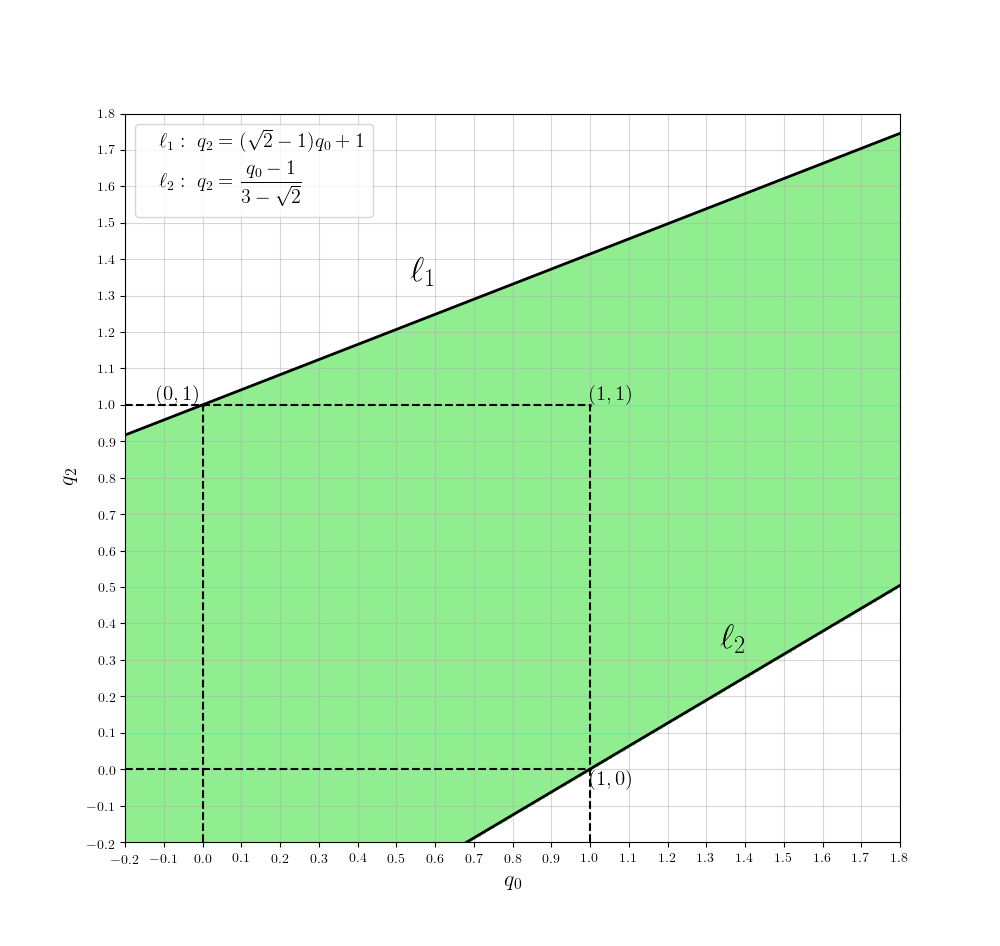
\includegraphics[width=\linewidth]{part_2/graf_3_1}
		\caption{$\mu = 0, \: \lambda \in [0, 1)$}
	\end{subfigure}
	\begin{subfigure}[b]{0.3 \textwidth}
		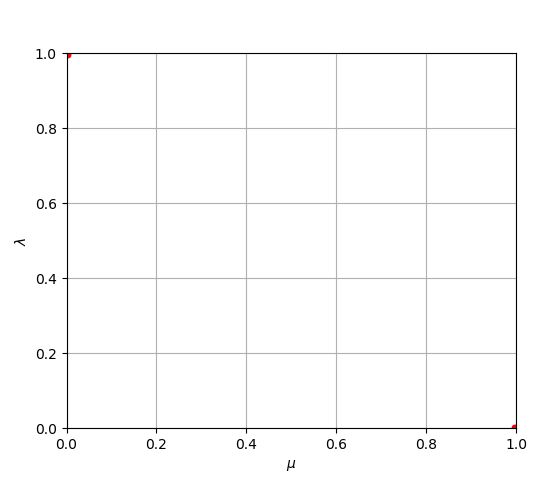
\includegraphics[width=\linewidth]{part_2/graf_3_2}
		\caption{
			$
			\left[
			\begin{array}{c}
     			\mu=0, \: \lambda = 1 \\
     			\mu=1, \: \lambda = 0
  			\end{array}
			\right.
			$
		}
	\end{subfigure}
	\begin{subfigure}[b]{0.3 \textwidth}	
		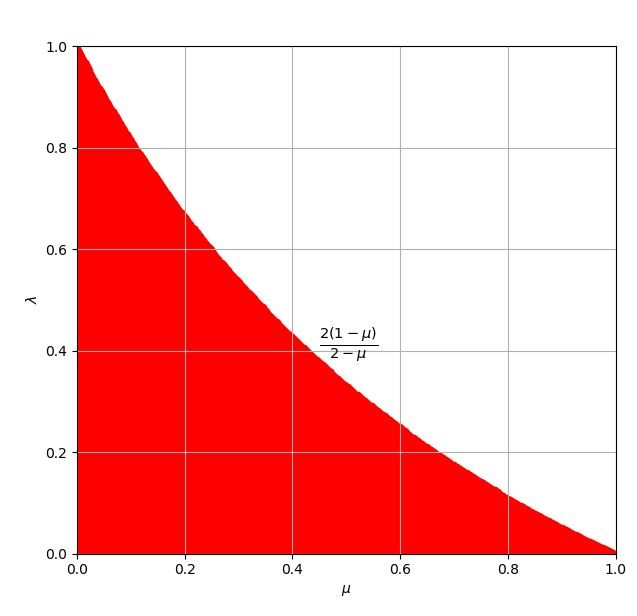
\includegraphics[width=\linewidth]{part_2/graf_3_3}
		\caption{
			$
				\mu \in (0,1), \:
				\lambda \in (0, \frac{1 - \mu}{1 + \mu}]
			$		
		}
	\end{subfigure}
	\caption{}
\end{figure}

\textbf{(1)} 
$\mu = 0, \lambda \in [0, 1):$
$$
	\begin{cases}
		p^* = 1 \\ 
		q^* = 0 
	\end{cases} \cup \quad
	\begin{cases}
		p^* = 1 \\
		q^* = \dfrac{\mu}{2-\mu} = \{\mu = 0 \} = 0
	\end{cases}
$$

Mножествo оптимальных стратегий 
$\mathbb{O} = \{ (1, 0) \}$

\hspace{5mm}

\textbf{(2.1)}
$\mu=0, \lambda =1:$
$$
	\begin{cases}
		p^* \geqslant 1 - \mu = \{\mu = 0\} = 1 \\
		q^* = \dfrac{\mu}{2 - \mu} = \{\mu = 0\} = 0
	\end{cases} \cup \quad
	\begin{cases}
		p^* \leqslant 1 - \mu = \{\mu = 0\} = 1 \\
		q^* = \dfrac{2\mu}{1 + \mu} = \{\mu = 0\} = 0 
	\end{cases}
$$

Mножествo оптимальных стратегий 
$\mathbb{O} = [0, 1] \times \{0\}$, где $\times$ - 
это декартово произведение.

\hspace{5mm}

\textbf{(2.2)}
$\mu = 1, \lambda = 0:$
$$
	\begin{cases}
		p^* \geqslant 1-\mu = \{\mu=1\}=0 \\
		q^* = \dfrac{\mu}{2-\mu} = \{\mu=1\}=1
	\end{cases} \cup \quad
	\begin{cases}
		p^* \leqslant 1 - \mu = \{\mu = 1\} = 0\ \\
		q^* = \dfrac{2\mu}{1 + \mu} = \{\mu = 1\} = 1 
	\end{cases}
$$

Mножествo оптимальных стратегий 
$\mathbb{O} = [0, 1] \times \{1\}$

\hspace{5mm}

\textbf{(3)}
$\mu \in (0,1), \lambda \in (0, \dfrac{1 - \mu}{1 + \mu}]$: 
$$
	\begin{cases}
		p^* = 1 \\ 
		q^* = \dfrac{\mu}{2 - \mu} 
	\end{cases}
$$

Mножествo оптимальных стратегий 
$\mathbb{O} = \{1\} \times \{\dfrac{\mu}{2-\mu}\}$ 

\begin{figure}[H]
	\centering
	\begin{subfigure}[b]{0.3 \textwidth}
		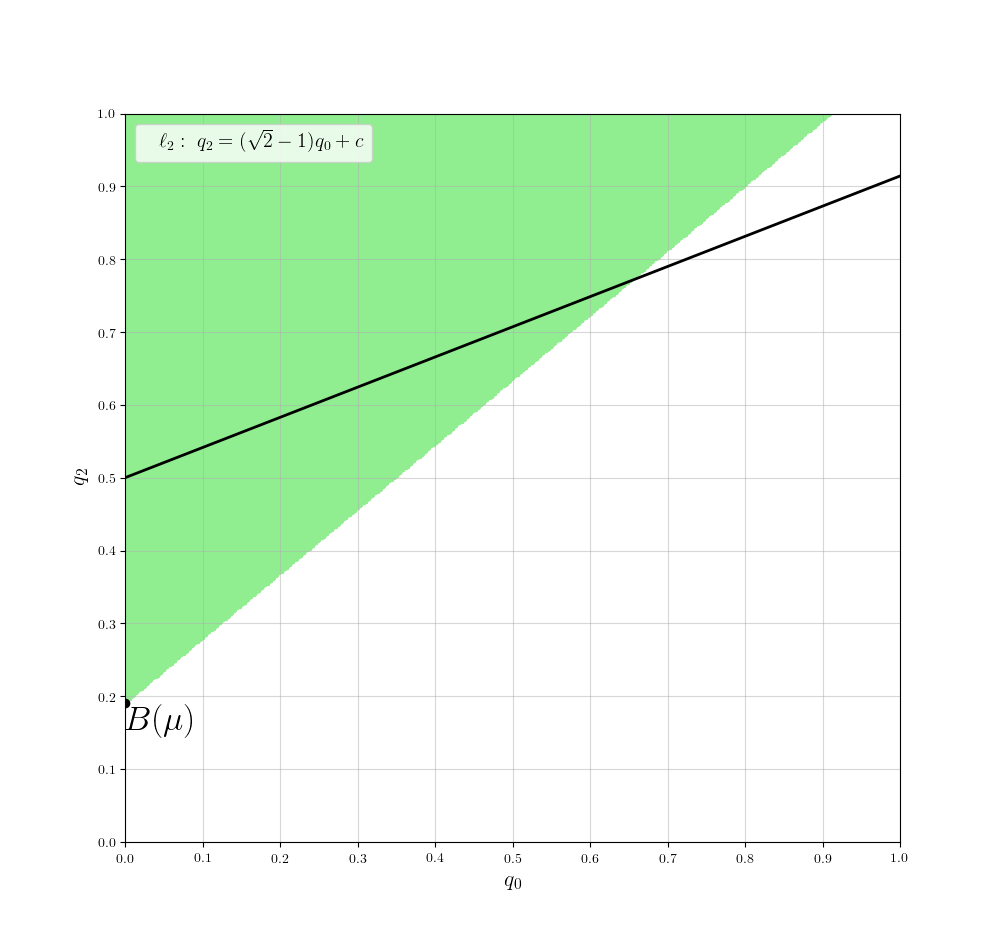
\includegraphics[width=\linewidth]{part_2/graf_3_4}
		\caption{
			$\mu \in (0,1), \lambda = \dfrac{1-\mu}{1+\mu}$		
		}
	\end{subfigure}
	\begin{subfigure}[b]{0.3 \textwidth}
		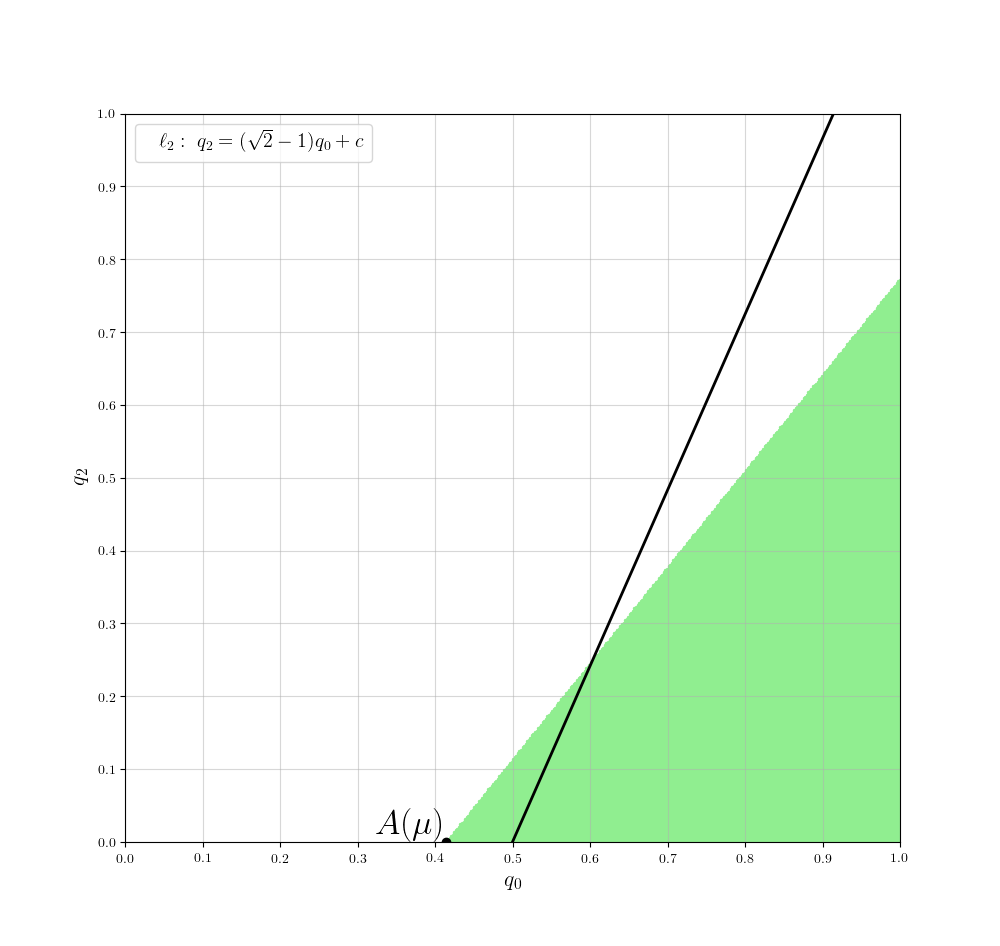
\includegraphics[width=\linewidth]{part_2/graf_3_5}
		\caption{
			$\mu \in [(, 1), \newline 
			\lambda \in 
			[0, 2\frac{1 - \mu}{2 - \mu}] \cap 
			(\frac{1 - \mu}{1 + \mu}, 1]$
		}
	\end{subfigure}
	\begin{subfigure}[b]{0.3 \textwidth}	
		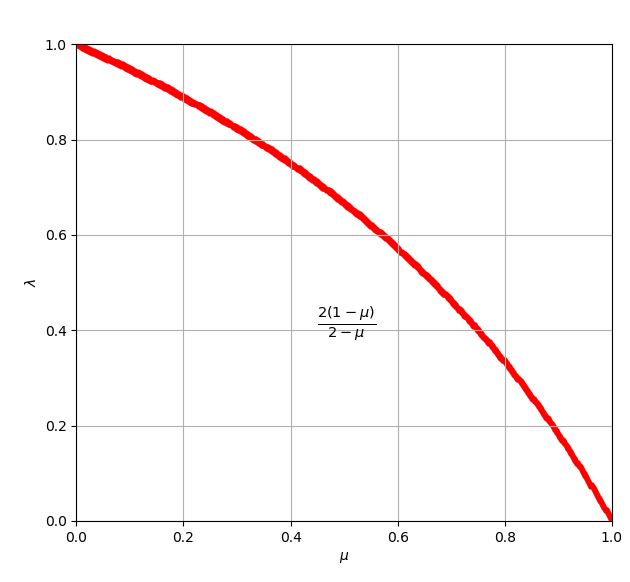
\includegraphics[width=\linewidth]{part_2/graf_3_6}
		\caption{
			$\mu \in (0, 1), \lambda = 2\dfrac{1 - \mu}{2 - \mu}$: 
		}
	\end{subfigure}
	\caption{}
\end{figure}

\hspace{5mm}

\textbf{(4)}
$\mu \in (0,1), \lambda = \dfrac{1-\mu}{1+\mu}$:
$$
	\begin{cases}
		p^* \in [0, 1 - \mu] \cup \{1\} \\
		q^* = \dfrac{\mu}{2 - \mu}
	\end{cases}
$$

Mножествo оптимальных стратегий 
$\mathbb{O} = \{1\} \times \{\frac{\mu}{2-\mu}\} \cup
[0,1-\mu] \times \{\frac{2\mu}{1+\mu}\}$ 

\hspace{5mm}

\textbf{(5)}
$\mu \in [(, 1), \lambda \in 
[0, 2\dfrac{1 - \mu}{2 - \mu}] \cap (\dfrac{1 - \mu}{1 + \mu}, 1]$: 
$$
	\begin{cases}
		p^* = 0 \\
		q^* = \dfrac{2\mu}{1 + \mu}
	\end{cases}  \cup \quad
	\begin{cases}
		p^* = 1 \\
		q^* = \dfrac{\mu}{2 - \mu}
	\end{cases}
$$

Mножествo оптимальных стратегий 
$\mathbb{O} = (0, \dfrac{2\mu}{1 + \mu}) \cup
(1, \dfrac{\mu}{2 - \mu})$ 

\hspace{5mm}

\textbf{(6)}
$\mu \in (0, 1), \lambda = 2\dfrac{1 - \mu}{2 - \mu}$: 
$$
	\begin{cases}
		p^* = 0 \\
		q^* = \dfrac{2\mu}{1 + \mu}
	\end{cases}  \cup \quad
	\begin{cases}
		p^* \in [0, 1 - \mu] \\
		q^* = \dfrac{\mu}{2 - \mu} 
	\end{cases}
$$

Mножествo оптимальных стратегий 
$\mathbb{O} =(0, \dfrac{2\mu}{1+\mu}) \cup
[1 - \mu, 1] \times \{\dfrac{\mu}{2 - \mu}\}$ 

\begin{figure}[H]
	\centering
	\begin{subfigure}[b]{0.4 \textwidth}
		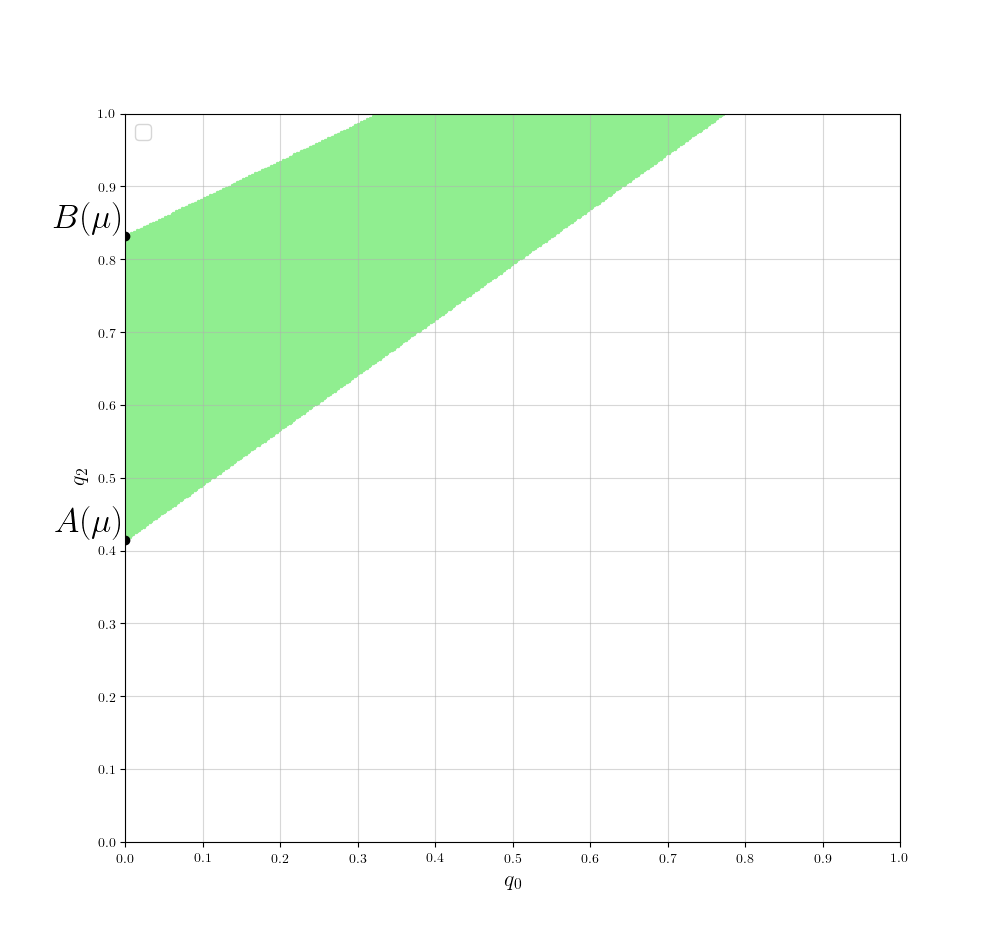
\includegraphics[width=\linewidth]{part_2/graf_3_7}
		\caption{
			$\mu \in (0, 1), 
			\lambda \in (2\dfrac{1 - \mu}{2 - \mu}, 1]$		
		}
	\end{subfigure}
	\begin{subfigure}[b]{0.4 \textwidth}
		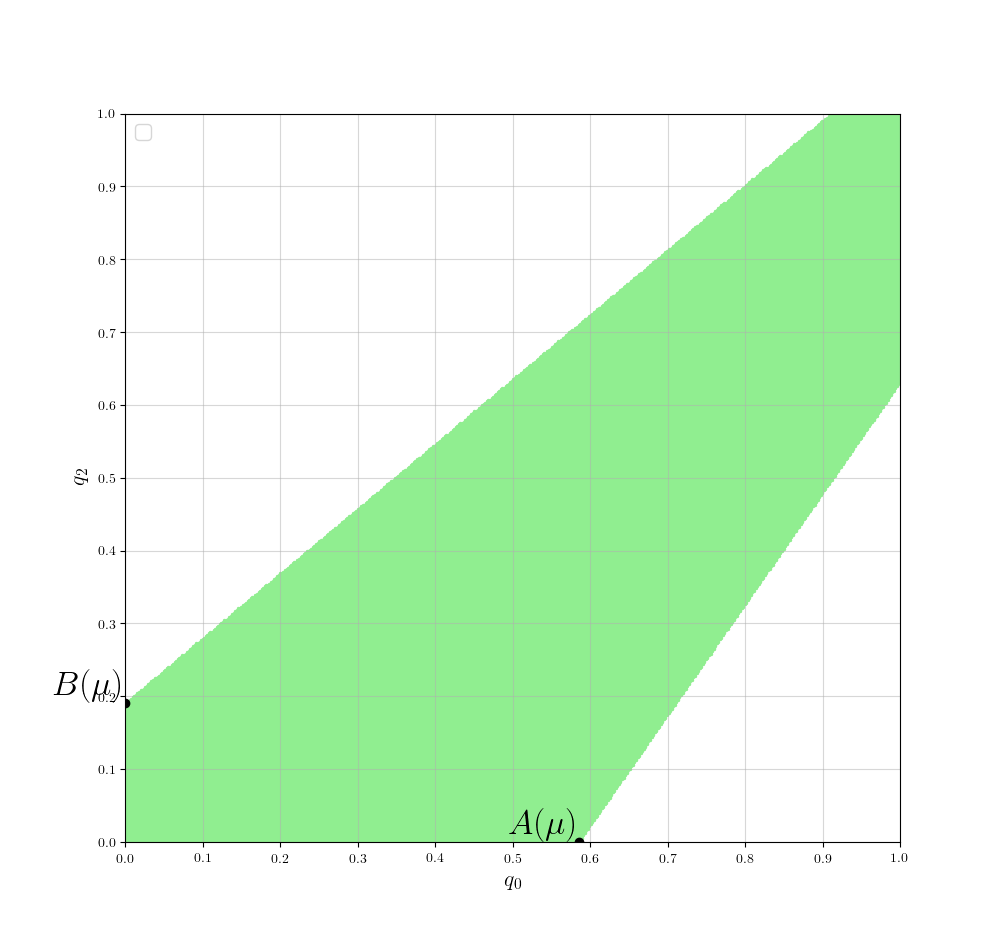
\includegraphics[width=\linewidth]{part_2/graf_3_8}
		\caption{
			$\mu = 1, \lambda \in (0, 1] $		
		}
	\end{subfigure}
	\caption{}
\end{figure}

\hspace{5mm}

\textbf{(7)}
$\mu \in (0, 1), \lambda \in (2\dfrac{1 - \mu}{2 - \mu}, 1]$: 
$$
	\begin{cases}
		p^* = 0 \\
		q^* = \dfrac{2\mu}{1 + \mu}
	\end{cases}
$$

Mножествo оптимальных стратегий 
$\mathbb{O}  = (0, \dfrac{2\mu}{1 + \mu})$

\hspace{5mm}

\textbf{(8)}
$\mu = 1, \lambda \in (0, 1] $: 
$$
	\begin{cases}
		p^* = 0 \\
		q^* = 1 \\
	\end{cases}  \cup \quad
	\begin{cases}
		p^* = 0 \\
		q^* = \dfrac{2\mu}{1 + \mu} = \{\mu = 1\} = 1 \\
	\end{cases}
$$

Mножествo оптимальных стратегий 
$\mathbb{O} =(0, 1)$ 
\end{flushleft}